\documentclass[10pt,conference]{IEEEtran}
\usepackage{lmodern}
\usepackage{amssymb,amsmath}
\usepackage{ifxetex,ifluatex}
\usepackage{multirow}
\usepackage{booktabs}
\usepackage{fixltx2e} % provides \textsubscript
\ifnum 0\ifxetex 1\fi\ifluatex 1\fi=0 % if pdftex
  \usepackage[T1]{fontenc}
  \usepackage[utf8]{inputenc}
\else % if luatex or xelatex
  \ifxetex
    \usepackage{mathspec}
  \else
    \usepackage{fontspec}
  \fi
  \defaultfontfeatures{Ligatures=TeX,Scale=MatchLowercase}
\fi
% use upquote if available, for straight quotes in verbatim environments
\IfFileExists{upquote.sty}{\usepackage{upquote}}{}
% use microtype if available
\IfFileExists{microtype.sty}{%
\usepackage{microtype}
\UseMicrotypeSet[protrusion]{basicmath} % disable protrusion for tt fonts
}{}
\usepackage{hyperref}
\PassOptionsToPackage{usenames,dvipsnames}{color} % color is loaded by hyperref
\hypersetup{unicode=true,
            pdftitle={CS229 Project Milestone},
            pdfauthor={Honghao Qiu},
            colorlinks=true,
            linkcolor=black,
            citecolor=Blue,
            urlcolor=Blue,
            breaklinks=true}
\urlstyle{same}  % don't use monospace font for urls
\usepackage{graphicx,grffile}
\makeatletter
\def\maxwidth{\ifdim\Gin@nat@width>\linewidth\linewidth\else\Gin@nat@width\fi}
\def\maxheight{\ifdim\Gin@nat@height>\textheight\textheight\else\Gin@nat@height\fi}
\makeatother
% Scale images if necessary, so that they will not overflow the page
% margins by default, and it is still possible to overwrite the defaults
% using explicit options in \includegraphics[width, height, ...]{}
\setkeys{Gin}{width=\maxwidth,height=\maxheight,keepaspectratio}
\IfFileExists{parskip.sty}{%
\usepackage{parskip}
}{% else
\setlength{\parindent}{0pt}
\setlength{\parskip}{6pt plus 2pt minus 1pt}
}
\setlength{\emergencystretch}{3em}  % prevent overfull lines
\providecommand{\tightlist}{%
  \setlength{\itemsep}{0pt}\setlength{\parskip}{0pt}}
\setcounter{secnumdepth}{5}
% Redefines (sub)paragraphs to behave more like sections
\ifx\paragraph\undefined\else
\let\oldparagraph\paragraph
\renewcommand{\paragraph}[1]{\oldparagraph{#1}\mbox{}}
\fi
\ifx\subparagraph\undefined\else
\let\oldsubparagraph\subparagraph
\renewcommand{\subparagraph}[1]{\oldsubparagraph{#1}\mbox{}}
\fi
\usepackage{subfig}
\AtBeginDocument{%
\renewcommand*\figurename{Figure}
\renewcommand*\tablename{Table}
}
\AtBeginDocument{%
\renewcommand*\listfigurename{List of Figures}
\renewcommand*\listtablename{List of Tables}
}
\usepackage{float}
\floatstyle{ruled}
\makeatletter
\@ifundefined{c@chapter}{\newfloat{codelisting}{h}{lop}}{\newfloat{codelisting}{h}{lop}[chapter]}
\makeatother
\floatname{codelisting}{Listing}
\newcommand*\listoflistings{\listof{codelisting}{List of Listings}}

\title{Multiview Human Synthesis From a Singleview}
\author{Si Wen (06246679), Tiancong Zhou (06247022), Honghao Qiu (06246258)\\
\texttt{\{wensi, longztc, honq\}{@}stanford.edu}}

% Begin custom, non-pandoc commands.

\newcommand{\latexonlyrule}{\rule}

% End custom, non-pandoc commands.

\begin{document}
\maketitle

\newcommand{\R}{\mathbb{R}}
\newcommand{\eqnset}[1]{\left.\mbox{$#1$}\quad\quad\right\rbrace}
\newcommand{\tr}{\text{tr}\;}
\renewcommand{\th}{\theta}
\newcommand{\toi}{^{(i)}}

%comments

\textbf{Abstract --  }
\textbf{We use deep generative models to synthesize multiview images given a single view. The generation process is done in two stages: in the first stage, we train a variational auto-encoder (VAE) to synthesize a new view of the input image; in the second stage, we use a generative adversarial network (GAN) to generate details on the output of the first stage. We evaluate our results using both qualitative and quantitative methods. One potential application is generating multiview images for e-Commerce products.}


\section{Introduction} 
Our project aims to use machine learning techniques to generate multi-view images of a person given a single view RGB image. With the advances of generative adversarial networks in recent years, we try to tackle the problem of multi-view full human body synthesis from a given view in any angle. If successful, this could enable many useful applications in fashion/E-Commerce websites and in the field of photo/video edition and content generation, for example, in Amazon cloth stores we can help provide 360-degree rotation view for customers given a single front-view image taken for the model. 

To achieve this goal, we use color images of human with clothes in different angles as input data, with both real world multiview fashion dataset from MVC [] and synthetic human images in 360-degree views generated from Fuse/Blender. Then we use deep neural network approach to generate output images from the inputs, where the model is trained in a two steps. Firstly, the condition image (human body in a specific angle) and the value of target angle (ex. 90 degree) are inputed into Variational Auto-Encoder to generate a coarse image output for the target view, and then this coarse image along with the condition image are both inputed into a Siamese Network to generate fine image output for the target view angle. The output image is compared with the ground truth image in target angle by a CNN discriminator, and the generative network is trained adversarially. 

The following image briefly illustrates this process.

\begin{figure}[htbp]
\centering
\includegraphics{Model.PNG}
\caption{Condition input image is firstly inputed into VAE to generate coarse view image for target angle, then it is inputed into GAN to generate fine view image for target angle.}
\end{figure}


\section{Related Work}
In recent years, there have been numerous attempts to solve subsets of this problem. 

On one hand, some previous research attempt to generate full human body image for some specific angles given the front view. For example, Zhao et al [2] proposed a VAE+GAN model to synthesize the side and back view of a person given the frontal view. This approach has the strength of combining the ability of VAE to find global appearance/outline and the ability of GAN to fill in fine details. This approach inspires us to try a very similar model pipeline. However, there are several limitations in their work: 1. in their paper, their model inputs the target image into VAE for generating coarse image output, where we want to get rid of this input, 2. due to the limitation of available data, their model only generates side and back view image outputs, and cannot be extended to output images for any target angle, 3. their work mainly focuses on the person’s clothing, and the resulting image contains poorly synthesized face. Our work would try to overcome these limitations.

On the other hand, some other researches work on generating specific areas of human, such as faces, hands, etc. instead of full human body, and still, due to the limitation of available data, the synthesis outputs are typically in limited views such as front/side/back view. For example, Huang et al [3] proposed a method to provide photorealistic synthesis of the frontal views of a person’s face given a side view. We try to leverage some of their loss functions that are helpful for face synthesis and include them into our method when we generate multiview images of an entire person.

There are some other related works for object rotation [6,8] (such as car/chair), and 3d model generation based on multiview images [3,5,6]. Some of their work [] has reached pretty good results for generating 360-degree synthesis by using [TODO: MODEL], but this task is relatively less difficult compared to multiview human and fashion synthesis since the target object output typically contains less details and simpler texture to be generated. 

\section{Dataset and Features}
Solving this problem requires large amount of training data for the network to learn the latent representation. We use a combination of real world datasets and synthetic datasets. We used a combination of MVC datasets (160,000 real images) and 80,000 synthetic images (360-degrees views). Image data are labeled with the associated angles for the view (ex. 60 degree).

Since the currently available real world views are rather limited and often only have frontal, back, and side views, we try to overcome this limitation by using 360-degree synthetic images generated from 3D modeling softwares. We also notice that some past usage of synthetic data on vision problems has shown promising results [2,5,6].

Our 360-degree human view dataset (about 100,000 full-body human images in 360-degree views) is generated by the following approach:
\renewcommand{\labelenumi}{\roman{enumi}}
 \begin{enumerate}
   \item Create 3D character models in Adobe Fuse. Adobe Fuse provides plenty of hairstyles, faces, cloth and shoes to combine and create 3D characters;
   \item Export the model as .obj file;
   \item Import the obj file into Blender. (Blender is a 3D graphics software that could be programmed and rendered to generate 360-degree views);
   \item Render and generate front view;
   \item Rotate the 3D character model by 1 degree clockwise, render and generate new view from that degree;
   \item Repeat step 5 and 6 until generating views for all 360 degrees.   
 \end{enumerate}

Examples of synthetic images we generated:

\begin{figure}[htbp]
\centering
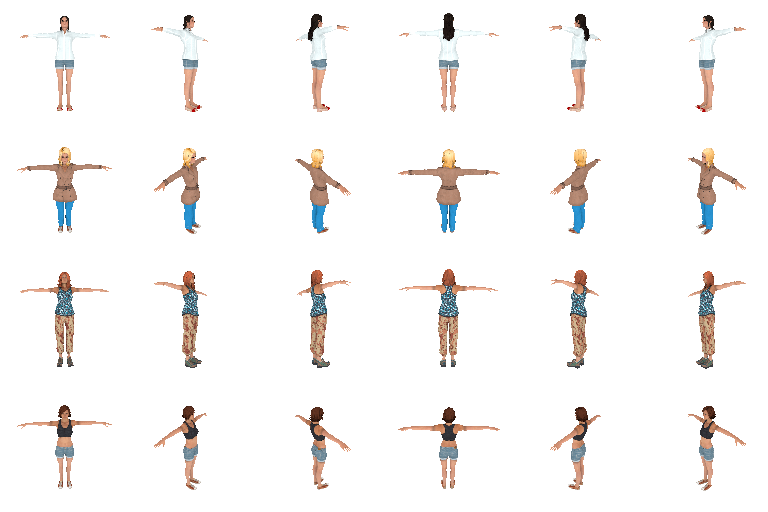
\includegraphics{data.png}
\caption{Synthetic Multiview Human Image Samples}
\end{figure}

Data Preprocessing:

//TODO

We use 1000 images for testing and the rest of data for training.



\section{Methods}

\subsection{Overview}

We tackle this problem using deep generative models. We divide our pipeline into two stages: the first stage consists of an input image, a target angle (0 to 360 degrees), and a conditional VAE. The encoder transforms the input image into a latent variable, concatenate it with the target angle, and passes them through the decoder. The decoded image should resemble the input image in the target angle, with noticeable artifact (e.g. blurry, sometimes with incorrect colors). The second stage consists of the original input image, output of the first stage (coarse image), and a conditional GAN. Both images are fed into a hierarchical feature extractor to obtain their latent representations. These latent representations are then concatenated and fed into a generator to obtain the final output. The generator is able to extract low level patterns from the original input image and generate a new image that conforms to the structure of the coarse image with patterns from the original input image.

\subsection{Variational Auto-Encoder (VAE)}

The VAE encodes the input image, concatenates it with
the target angle (scalar value in [0, 360]), and feeds them
through the decoder to produce an image in the target view.

We feed the input image and the output from VAE
through a Siamese network to produce the final fine image
in the target view, and is trained adversarially.

\subsection{Generative Adversarial Network (GAN)}


\subsection{Pipeline Overview}
We combines variants of the Generative Adversarial Network (GAN) [1] to solve this problem. GAN is a generative approach that learns a distribution to represent the training data. We can then generate new images sampled from that distribution, conditioned on the input image and the desired angles. Here is a picture illustrating our pipeline.

\begin{figure*}[htbp]
\centering
\includegraphics{Picture2.png}
\caption{Pipeline Overview}
\end{figure*}

As is shown in Zhao et al paper [VariGan, 2], GAN is good at filling rich details of the synthesized image but less capable of capturing global appearance and rough outlines for human/clothings, and on the other hand, VAE [7] is more capable of finding global appearance with less detailed details, therefore, GAN and VAE are good complements of each other for image synthesis. Our model follows the following two-step approach to achieve image synthesis: 1) firstly use VAE to model coarse global appearance (outline/structure of the image), 2) then use variants of GAN to model refined details of the person and get fine synthesized images of full human body in multiviews. Compared to Zhao's model, we did not input the target image into VAE, but instead only input conditional image and the target angle to VAE model. Another improvement we are making is, with our synthetic data for human body from all angles, we target at outputting all 360-degree multiview human synthesis from a given view of any angle. This is achieved by changing the angle degree input in the VAE model during training process according to the label of target output image (i.e. the target angle). 

Furthermore, one potential reason why VariGAN approach has a poor performance on head synthesis might be only adversarial loss being used in GAN's objective. Inspired by Huang et al's work [3], we try to model face generation better by using pixel to pixel comparison loss, in this way face features would be better captured since incorrectly predicted faces are penalized with additional loss (more details are discussed in Objective Function section).

\subsection{Network Architecture}
\textbf{VAE Architecture} 
We use 6 convolution layers in the VAE encoder 

\textbf{GAN Architecture} 


\subsection{Objective (Loss) Function}
We mainly use the following loss functions (with penalty factor assigned to each loss and calculating the combined loss as objective loss function):

\begin{itemize}
\item Adversarial loss:\\
Without considering the conditional image (as is mentioned in model section), we define adversarial loss as:
$$ E_{I_v \sim p_{data(I_v)}}[log D(I_v)] + E_{z \sim p(z)}[log (1- D(I_v, G(z, I_v)))], $$
here $I_v$ stands for Image given a Viewpoint, D is the discriminator and G is the generator to be trained simultaneously.

\item VAE loss:\\
As is shown in Bowman et al's work [11], we are also using the standard VAE loss term, which is defined as the sum of KL-divergence loss and another posterior Expectation loss term:
$$ L(\theta;x)= -KL(q_\theta(z|x)||p(z))+E_{q_\theta(z|x)}[log(p_\theta(x|z))] $$

\item Pixel to pixel loss:\\
The pixel-wise loss can be expressed as [3]:
$$ \frac{1}{L*H} \sum_{x=1}^L \sum_{y=1}^H |\hat{I}_{x,y}- I_{x,y}|, $$
where L stands for Length (number of pixels in row-wise), and H stands for Height (number of pixels in column-wise). $\hat{I}_{x,y}$ is the predicted pixel of the image and $I_{x,y}$ is the corresponding pixel in GT.

\item Regularization term in loss function:\\
We use adaptive L2 regularization on the discriminator to penalize large weights and mitigate over-fitting. As is shown in [1], this is helpful when discriminator is too strong for the generator and the regularization term can be decreased when generator catches up with the discriminator.

\end{itemize}


\subsection{Implementation Details}

We implemented the VAE from scratch, and gradually 

\begin{figure}[htbp]
\centering
\includegraphics{experiments.png}
\caption{Row 1-4: output of VAEs with (1) fully-connected layers only with insufficient amount of  hidden neurons (2) fully-connected layers only with sufficient hidden neurons (3) convolutional layers with insufficient amount of filters (4) convolutional layers with sufficient amount of filters. }
\end{figure}

We attempted to implement a GAN from scratch. However, 

\section{Experimentation Results}







\begin{figure}[htbp]
\centering
\includegraphics{PICTURE4.png}
\caption{Output Image Results (using real world MVC dataset)}
\end{figure}

We use both quantitative and qualitative measures to assess the result of our work. 
We  start our project by generating side-view images from a frontal synthetic image, and then move to real images. We then try to generate views from all angles, including the ones where one cannot easily infer the person’s look from the frontal image (e.g. the back of the head, hair, cloth, etc). Given time, we will also try solving the problem under different lighting and background conditions. The performance of the model output would be judged by both loss comparison with previous models, and by comparison results provided by a set of human judges. We would also conduct algorithmic analysis to find out the impact of each component of our networks (GAN, VariGAN, TPGAN, VAE, etc.) and the contribution of each type of training datasets (real images, synthesized images in front, back, and side views, etc.).

Here is the current preliminary result of our model output for human synthesis in different angles (using VAE without conditional image input, 200 filters and 10000 training images for each layer, based on MVC and DeepFashion Dataset). We use this simple VAE model as the  baseline model and compare other modeling results with the baseline performance to observe the improvement. As is shown in the picture, currently, our model is able to synthesize roughly the structure and color for human body in different angles, but it lacks the details to make it high resolution, and we are also having difficulty to ensure that the synthesized images are always rotated.



We use several different quantitative methods to evaluate the quality of our model, including the Structural Similarity Index (SSIM) and the Inception Score (IS).
\begin{itemize}


\item SSIM:\\
Structural Similarity:
$$SSIM(I_x,I_y)=\frac{(2\mu_x \mu_y + c_1)(2\sigma_{xy}+c_2)}{(\mu_x^2+\mu_y^2 +c_1)(\sigma_x^2+\sigma_y^2+c_2)}$$

\item IS:\\
Inception Score:
$$IS(I_x,I_y)=exp(E_{I_x}D_{KL(p(y|I_x)||p(y))})$$
where $I_x,I_y$ are generated image and GT image respectively, and y is the label (the input angle in our model).

\item RMSE:\\
Root Mean Square Error:


\end{itemize}

\begin{figure*}
  \includegraphics[width=\linewidth]{FigureTable.PNG}
  \caption{Experimental Results}
  \label{fig:boat1}
\end{figure*}

\section{Discussions and Future Work}

Discussion:

1. Our model works well on synthetic images, as there are less noise in the data (e.g. no background, unified pose, similar texture, etc.).

2. On MVC dataset, we achieved reasonably good result compared to other methods (see table above). Since VAE is capable of finding 
global appearance with less details, while GAN is good at filling rich details of the synthesized image but less capable of capturing 
global appearance and rough outlines for human/clothings, therefore, GAN and VAE complements each other well for image synthesis 
in our architecture. The coarse image generated by VAE captures global appearance, while GAN fills in details to make the fine image.

3. Our model does not perform well on face synthesis (compared to the body), since face contains more details and is harder to synthesize.

Future work:

1. Improve the GAN: we only used a simple conditional GAN with very little hyperparameter tuning. There is a number of recently published papers that shows various techniques to improve the quality and stability of GANs.

2. Improve face synthesis: our model currently handles face poorly since it contains a lot of noticeable details. It is important to be able to recreate these details in a convincing way for good result. 

3. Include background: our current dataset only contains images without any background. It is more difficult to synthesize views when the object of interest is not presented in isolation and we would like to tackle that problem in the future.


In the future, we would use all images in our self-generated datasets and combine the current GAN model with VAE models, along with TPGAN for better face/head synthesis, to achieve a better synthesis model performance for human body. For the low resolution difficulty, we hope to solve this by introducing variants of GANs and longer training time with more training data to better learn the latent representation of the picture. We also plan to try introducing conditional image (i.e. both using target image and the conditional image in two different views) for encoder input, in order to achieve a better rotational result for our human body synthesis.


\section{Conclusion}
We aims at solving 360-degree full human body view synthesis problem by using our self-generated dataset and VAE+GAN modeling approach, while introducing some minor changes on modeling architecture and loss function compared with previous works [1,2,3].
Current preliminary results show some promising potential of our modeling approach. With the help of large volume self-generated human view data from 360 view angles, we hope we can solve the 360 degree full human body view synthesis problem and achieve state-of-art results.

\textbf{Teammate Contributions:}

Our teamwork break down:
\begin{itemize}
\item Si (Vincent) Wen: Vicent is mainly working on variants of GAN modeling, he also contributed to dataset generation (Fuse and MVC) and writing reports (some of modeling section). He is also working on TPGAN to improve the model performance.
\item Tiancong Zhou: Tiancong is mainly working on dataset generation (human viewed from 360 degrees in Blender), he also contributed to the report (some of data description section) and modeling part with regards to data processing.
\item Honghao Qiu: Honghao is mainly working on modeling and reporting. He works on VAE+GAN modeling, and he is the main contributor to writing this report, he is also engaged in data collection (Deep Fashion).
\end{itemize}

Our team target at equal contributions from three team members across data, modeling, and reporting.  In general, all our teammates have made equal contribution to this project so far. We hope to successfully finish the project with our collective efforts!

\section{References}

[1] Goodfellow et al, Generative Adversarial Nets, $https://arxiv.org/pdf/1406.2661.pdf$ 

[2] Zhao et al, Multi-View Image Generation from a Single-View, $https://arxiv.org/pdf/1704.04886.pdf$

[3] Huang et al, Beyond Face Rotation: Global and Local Perception GAN for Photorealistic and Identity Preserving Frontal View Synthesis, $https://arxiv.org/pdf/1704.04086.pdf$ 

[4] Yim et al, Rotating Your Face Using Multi-task Deep Neural Network, $https://www.cv-foundation.org/openaccess/content_cvpr_2015/papers/-Yim_Rotating_Your_Face_2015_CVPR_paper.pdf$

[5] Ashish et al, Learning from Simulated and Unsupervised Images through Adversarial Training, $https://arxiv.org/abs/1612.07828$

[6] Rajpura et al, Object Detection Using Deep CNNs Trained on Synthetic Images, $https://arxiv.org/pdf/1706.06782.pdf$

[7] Diederik et al, Auto-Encoding Variational Bayes, $https://arxiv.org/pdf/1312.6114.pdf$

[8] Kihyuk et al, Learning Structured Output Representation using Deep Conditional Generative Models, $https://pdfs.semanticscholar.org/3f25/-e17eb717e5894e0404ea634451332f85d287.pdf$

[9] IJCAI 2017, NEU, Fashion Style Generator, $https://www.ijcai.org/proceedings/2017/0520.pdf$

[10] NIPS 2017, ETH/MPII, Pose Guided Person Image Generation, $https://arxiv.org/pdf/1705.09368.pdf$

[11] Bowman et al, Generating Sentences from a Continuous Space, $https://arxiv.org/pdf/1511.06349.pdf$

[12] MVC Fashion Dataset, $http://mvc-datasets.github.io/MVC/$

[13] Deep Fashion Dataset, $http://mmlab.ie.cuhk.edu.hk/projects/DeepFashion.html$

\end{document}
